
% ######################################################################### %
% ------------------------------------------------------------------------- %
%                     Degree distribution
% ------------------------------------------------------------------------- %
% ######################################################################### %

\section{Degree distribution}\label{sec:degree_distribution}


The in- and out-degree of a vertex in a directed graph describes the
number of incoming and outgoing connection from and to other
\marginpar{cf. Definition~\ref{def:in_out_degree}} vertices. As a
fundamental concept in graph and network theory, the degree
distribution is integral in the categorization of networks and allows
for the estimation of graph properties. 

Node degree distribution was shown to have strong impact on the
dynamics of neuronal networks models commonly used in computational
neuroscience research \parencite{Roxin2011}. Increasing in-degree
variance for example could be connected to the appearance of
oscillations in the network. Extracting degree distributions from
biological networks however, remains a challenge as many neurons need
to be tracked simultaneously to obtain enough data to confidently
estimate degree distributions.

\begin{figure}[H]
  \centering
  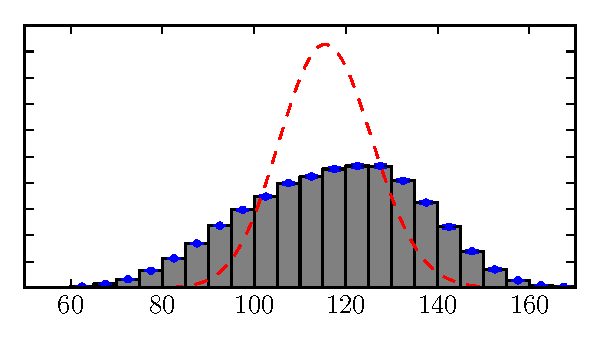
\includegraphics[width=0.65\textwidth]{%
    plots/9326138e.pdf}
  \caption{\textbf{In-degree distribution in anisotropic networks
      shows comparably high variance and is skewed to the left} From 250
    anisotropic networks in-degree distributions were extracted and
    are shown in a normed histogram plot, errorbars SEM. Comparison with the
    binomial degree distribution (red) of a Gilbert random graph model
    with matching parameter set ($N=1000$, $p =0.116$) shows higher
    variance of in-degrees in anisotropic networks (sample variance $=
    344.54$, variance of binomial distribution $Np(1-p) = 102.44$.)
    Skewness to the left of the sample is $-0.1763.$
    (\smtcite{9326138e})}
  \label{fig:in_degree_ER_compare}
\end{figure}

Here we analyze in- and out-degrees in the anisotropic network
model. First we find that compared to the binomial in-degree
distribution of a Gilbert random graph model, in-degrees of vertices
in anisotropic networks display higher variance and their distribution
is skewed to the left (\autoref{fig:in_degree_ER_compare}). However,
this specific in-degree profile is not an intrinsic property of
anisotropy, as the distribution remains stable under manipulation of
the anisotropy degree and closely matches the profile of a purely
distance-dependent network (\autoref{fig:in_degree_rewiring}). This
result agrees with findings of \textcite[Fig. S3]{Perin2011}, who were
able to recreate degree distributions from their experiment with layer
5 thick-tufted pyramidal cells in neonatal rats from the extracted
distance-dependent connection profiles alone.

\begin{figure}[H]
  \centering
  \renewcommand{\tabcolsep}{2pt}
  \setlength\extrarowheight{0pt}
  \begin{tabular}{lll}
    \begin{overpic}[width=0.28\textwidth]{%
        plots/77995b6b_in000.pdf}
      \put(12,56){\small $\eta = 0$}
    \end{overpic}
    &
    \begin{overpic}[width=0.28\textwidth]{%
        plots/77995b6b_in025.pdf}
      \put(12,56){\small $\eta = 0.25$}
    \end{overpic}
    &
    \begin{overpic}[width=0.28\textwidth]{%
        plots/77995b6b_in050.pdf}
      \put(12,56){\small $\eta = 0.5$}
    \end{overpic}
    \\
    \begin{overpic}[width=0.28\textwidth]{%
        plots/77995b6b_in075.pdf}
      \put(12,56){\small $\eta = 0.75$}
      \put(4,-4){\small$0$}\put(78,-4){\small$200$}
    \end{overpic}
    &
    \begin{overpic}[width=0.28\textwidth]{%
        plots/77995b6b_in100.pdf}
      \put(12,56){\small $\eta = 1$}
      \put(4,-4){\small$0$}\put(78,-4){\small$200$}
    \end{overpic}
    & 
    \begin{overpic}[width=0.28\textwidth]{%
        plots/77995b6b_indst.pdf}
      \put(12,56){\small distance}
      \put(4,-4){\small$0$}\put(78,-4){\small$200$}
    \end{overpic}
    \\
  \end{tabular}
  \caption{\textbf{In-degree distribution not affected by varying
      degrees of anisotropy} In-degree distributions from the 25
    sample graphs and their rewiring stages are plotted in normed
    histograms and listed from rewiring factor $\eta =0$ (original
    anisotropic) to $\eta = 1$ (completely rewired, maximal
    isotropy). Comparison shows that varying degrees of anisotropy do
    not influence the degree distribution, in fact in-degree
    distributions match with the degree distribution of an equivalent
    distance-dependent network shown bottom-right
    (\smtcite{77995b6b}). }
  \label{fig:in_degree_rewiring}
\end{figure}


While the out-degree distribution of vertices in the anisotropic
network also shows itself stable under rewiring, its distribution is
drastically different from the out-degree distribution in a comparable
distance-dependent network (\autoref{fig:out_degree_rewiring}). The
asymmetric, long-tailed distribution is identified as an artifact of
the anisotropic network's spatial confinement; a neuron, closely
located near a surface edge, might have an axon projection out of the
square causing minimal out-degree or, projecting through the entire
length of the surface, may have maximal out-degree. Approximating the
expected number of outgoing connections for a vertex in an anisotropic
network of size $N$, side-length $s$ and axon width $w$ as
\[
  N \frac{w l}{s^2},
\]
with parameters $N = 1000$ and $\frac{w}{s} = 0.252$, we obtain an
upper bound for the expected out-degree, 
\[
  N \frac{w l}{s^2} \leq N\frac{w}{s} \sqrt{2} \approx 350.
\]
If $f(l)$ is the probability density function to find axon length $l$
for a random node $v$ in the anisotropic network model, the out-degree
distribution is then approximated by
%
\begin{align}\label{eq:axon_length_approx}
  \mathbf{P}(d_{\mathrm{out}}(v) = N \frac{w l}{s^2}) = f(l),  
\end{align}
%
see also \autoref{fig:out_degree_ER_compare}.

\begin{figure}[H]
  \centering
  \renewcommand{\tabcolsep}{2pt}
  \setlength\extrarowheight{0pt}
  \begin{tabular}{lll}
    \begin{overpic}[width=0.28\textwidth]{%
        plots/77995b6b_out000.pdf}
      \put(12,56){\small $\eta = 0$}
    \end{overpic}
    &
    \begin{overpic}[width=0.28\textwidth]{%
        plots/77995b6b_out025.pdf}
      \put(12,56){\small $\eta = 0.25$}
    \end{overpic}
    &
    \begin{overpic}[width=0.28\textwidth]{%
        plots/77995b6b_out050.pdf}
      \put(12,56){\small $\eta = 0.5$}
    \end{overpic}
    \\
    \begin{overpic}[width=0.28\textwidth]{%
        plots/77995b6b_out075.pdf}
      \put(12,56){\small $\eta = 0.75$}
      \put(4,-4){\small$0$}\put(78,-4){\small$350$}
    \end{overpic}
    &
    \begin{overpic}[width=0.28\textwidth]{%
        plots/77995b6b_out100.pdf}
      \put(12,56){\small $\eta = 1$}
      \put(4,-4){\small$0$}\put(78,-4){\small$350$}
    \end{overpic}
    & 
    \begin{overpic}[width=0.28\textwidth]{%
        plots/77995b6b_outdst.pdf}
      \put(52,56){\small distance}
      \put(4,-4){\small$0$}\put(78,-4){\small$350$}
    \end{overpic}
    \\
  \end{tabular}
  \caption{\textbf{Out-degree distribution not affected by varying
      anisotropy but highly different from distance-dependent
      networks} Out-degree distributions from the 25 sample graphs and
    their rewiring stages are plotted in normed histograms and listed
    from rewiring factor $\eta =0$ (original anisotropic) to $\eta =
    1$ (completely rewired, maximal isotropy). While varying degrees
    of anisotropy do not influence the degree distribution, the
    characteristic out-degree profile is drastically different from
    the distribution found in equivalent distance-dependent networks
    (\smtcite{77995b6b}). }
  \label{fig:out_degree_rewiring}
\end{figure}


%------------------------------------------------
\marginpar{\vspace{1.91cm}\\Steep incline for small out-degree cut off
  due to binning (cf. \autoref{suppfig:out_degree})} 
%------------------------------------------------
\begin{figure}[H]
  \centering
  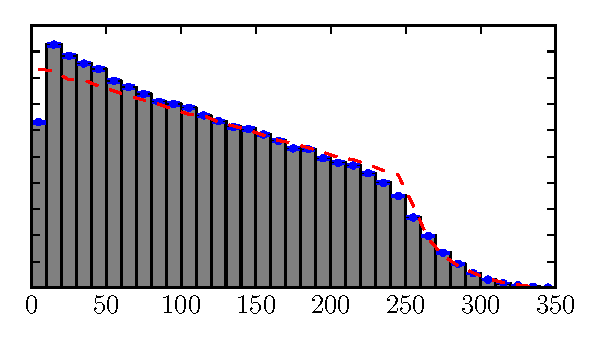
\includegraphics[width=0.65\textwidth]{%
    plots/019555b0.pdf}
  \caption{\textbf{Characteristic out-degree distribution as an
      artifact of network's boundaries} From 250 anisotropic networks
    out-degree distributions were extracted and are shown in a normed
    histogram plot, errorbars SEM. The characteristic distribution is
    identified as an artifact of the network's spatial confinement;
    using equation~\ref{eq:axon_length_approx} the out-degree profile
    is approximated (red) by the distribution of axon lengths in the
    anisotropic network (\smtcite{019555b0}).}
  \label{fig:out_degree_ER_compare}
\end{figure}



%%% Local Variables: 
%%% mode: latex
%%% TeX-master: "../dplths_document"
%%% End: 
